\documentclass{article}

% if you need to pass options to natbib, use, e.g.:
% \PassOptionsToPackage{numbers, compress}{natbib}
% before loading nips_2017
%
% to avoid loading the natbib package, add option nonatbib:
% \usepackage[nonatbib]{nips_2017}

\usepackage{nips_2017}

% to compile a camera-ready version, add the [final] option, e.g.:
% \usepackage[final]{nips_2017}

\usepackage[utf8]{inputenc} % allow utf-8 input
\usepackage[T1]{fontenc}    % use 8-bit T1 fonts
\usepackage{hyperref}       % hyperlinks
\usepackage{url}            % simple URL typesetting
\usepackage{booktabs}       % professional-quality tables
\usepackage{amsfonts}       % blackboard math symbols
\usepackage{nicefrac}       % compact symbols for 1/2, etc.
\usepackage{microtype}      % microtypography
\usepackage{graphicx}
\usepackage{subcaption}

\title{Reinforcement learning for pole balancing based on haptic feedback}

% The \author macro works with any number of authors. There are two
% commands used to separate the names and addresses of multiple
% authors: \And and \AND.
%
% Using \And between authors leaves it to LaTeX to determine where to
% break the lines. Using \AND forces a line break at that point. So,
% if LaTeX puts 3 of 4 authors names on the first line, and the last
% on the second line, try using \AND instead of \And before the third
% author name.

\author{
%  Hanjun Song\thanks{Use footnote for providing further
%    information about author (webpage, alternative
%    address)---\emph{not} for acknowledging funding agencies.} \\
%  Department of Computer Science and Engineering\\
%  University of Washington\\
%  Seattle, WA 98185 \\
%  \texttt{hanjuns@cs.uw.edu} \\
  %% examples of more authors
  %% \And
%   Hanjun Song \\
%   Department of  \\
%   Address \\
  %% \texttt{email} \\
  %% \AND
  %% Coauthor \\
  %% Affiliation \\
  %% Address \\
  %% \texttt{email} \\
  %% \And
  %% Coauthor \\
  %% Affiliation \\
  %% Address \\
  %% \texttt{email} \\
  %% \And
  %% Coauthor \\
  %% Affiliation \\
  %% Address \\
  %% \texttt{email} \\
}

\begin{document}
% \nipsfinalcopy is no longer used

\maketitle

\begin{abstract}
 
Conventional pole balancing problem is getting feedback of tilting angle (and the angular velocity) of the pole and the position (and the velocity) of the balancer. Also, the pole is kinematically constrained to the hinge of the balancer on 2 dimensional surface. In this paper, model-free reinforcement learning is used to implement pole balancing controller based on contact force feedback in 3 dimensional space. Natural policy gradient algorithm is used to learn the control policy. Pole balancing can be thought as one kind of non-prehensile manipulation and this paper shows the importance of reinforcement learning and the haptic feedback in non-prehensile manipulation.

\end{abstract}

\section{Introduction}

\subsection{Background}

People use a lot of strategies to manipulate object. One common example is grasping objects and move around. However, most of the manipulation is non-prehensile manipulation, which means manipulation not involving grasping. Non-prehensile manipulation includes actions such as balancing, pushing, pulling, flipping, throwing, and so on. Non-prehensile manipulation is challenging in robotics because of many reasons. To mention a few of them, non-prehensile manipulation couples grasp planning and kinematic motion planning and increases uncertainty of feedback from sensors. For example, occlusion occurs due to the robot hand when the robot uses visual feedback from the camera on the its head. Because the robot is not grasping the object, the uncertainty increases more than when the robot is grasping the object. Therefore, haptic feedback is required to have more stable feedback than visual feedback.

Haptic feedback is the combination of kinaesthetic feedback and tactile feedback. For robotic manipulators, kinaesthetic feedback is obtained by forward dynamics based on the torques of each joints or force/torque sensor on the end-effector. Tactile feedback is acquired by sensors which are able to sense normal force, shear force, and vibration. For humans, the sense of touch is a key factor that enables manual dexterity for humans. Accordingly, there have been a lot of attempts to develop robust and multi-modal tactile sensors for robots and reliable results came out recently. For example, GelSight and FingerVision are camera-based tactile sensors and they give not only force and vibration data, but also proximity visual data. In addition to the tactile sensor, sensitive torque control became available for actuators. For instance, HEBI Robotics developed a series-elastic actuator with 0.01Nm torque resolution. In this paper, ATI Nano 25 force/torque sensor is considered as a kinaesthetic feedback due to the high performance of the sensor. 

\subsection{Statement of the Problem}

Can robot balance a pole not based on the tilting angle, but based on the contact forces? What kind of reinforcement algorithm should be used to learn the control policy of this control problem? How can I transfer from simulation to physical system?

\subsection{Objectives}

The objectives of this research is to implement an algorithm for learning control policies of haptic-based pole balancing. This can be extended to non-prehensile problem as pole balancing is one kind of non-prehensile manipulation. The eventual goal of this research is to investigate the importance and possibility of haptic feedback in non-prehensile manipulation. Also, this research explores the way to transfer simulation to physical simulation by setting up the simulation environment as close as possible to the physical system.

%\subsection{Literature Review}


%The original motivation of this project stems from a pole balancing problem. Conventional pole balancing problems are based on visual feedback of the pole to estimate the leaning angle or angular feedback based on the encoder values at the joint of the pole and the base. However, those feedback controls restricts the shape of objects or requires specific hardware settings. To expand the type of objects from the pole to general shapes of objects, haptic feedback seems to be possible solution because it depends only on the contact forces. Also, reinforcement learning is essential to implement the control strategy for the physically unknown objects.
%
%To reduce the complexity of the problem, this problem can be thought on the two dimensional surface. Interestingly, two dimensional object balancing can be considered as a non-prehensile manipulation problem using pushing action. For example, a manipulator can be commanded to move an object using pushing action on a straight line based on the haptic feedback. This simplification reduces the states space from 6 degrees-of-freedom (DOF) to 3 DOF, but adds the uncertainty of the friction between the object and the surface. 
%
%Due to the advancement of the haptic sensors, such as tactile sensors, it seems to be feasible to tackle this problem in real world. Once the control strategy is trained on a simulation, such as MUJOCO, it will be tested on a 5 DOF manipulator with a tactile sensor.

%\subsection{Style}
%
%\subsection{Retrieval of style files}


\section{Methodology}

For the reinforcement algorithm, natural policy gradient algorithm is used to learn the control policy. Simulation environment with the similar parameters with the physical system is set up using MuJoCo. In MuJoCo simulation, a balancer (10cm x 10cm) is set to move on 2 dimensional surface and a pole (30cm x 1,2cm) is set to move in 3 dimensional space as a freejoint. On the balancer, 3 axis force sensor is added to sense the force at the contact between the balancer and the pole. The gear number of the motor in the simulation is adjusted from 7.0 to 3.0. 

For the natural policy gradient algorithm, position, velocity, and acceleration of the balancer and the contact forces are observed as states. In addition to that, rewards are given as a sum of the rewards for tilting angle and distance from the center and the penalty on control cost. Action is given as a 2 dimensional position of the balancer. Basically, the natural policy gradient algorithm learns the mapping from the observed balancer states and the contact forces to the position of the balancer in order to balance the pole.  For the convergence of the learning, learning parameters, such as the number of iterations and trajectories, should be adjusted depending on the physical parameters of the pole and the balancer. 

\begin{table}[h!]
\centering
  \begin{center}
  \begin{tabular}{ |p{3cm}|p{3cm}|p{3cm}| }
  \hline
  States & Rewards & Actions\\
  \hline  
  position, velocity, acceleration of the balancer, Contact forces & Tilting angle, Distance between the pole and the center, Penalty on control cost & Position of the balancer\\
  \hline
  \end{tabular}
  \end{center}
  \caption{States, Rewards, Actions of the algorithm}
  \label{table:1}
\end{table}

Eventually, the balancer should be able to balance the random objects with random inertia and shapes, but only capsule shapes of objects with different size and mass are considered in this paper to verify the feasibility of haptic based balancing. The adjusted parameters are the length, radius, and the mass of the capsule object in MuJoCo.

\begin{figure}[h!]
  \centering
  \begin{subfigure}[b]{0.4\linewidth}
    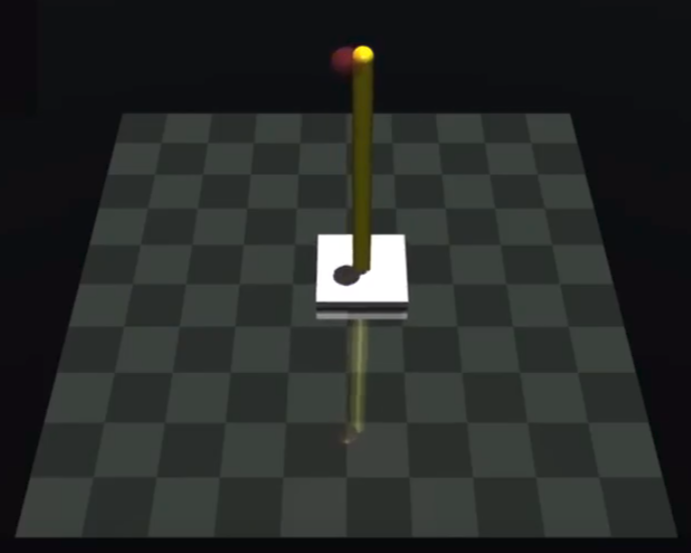
\includegraphics[width=\linewidth]{./Figures/pole_30_1.png}
    \caption{pole length:30cm, radius:1cm, mass:400g}
  \end{subfigure}
  \begin{subfigure}[b]{0.422\linewidth}
    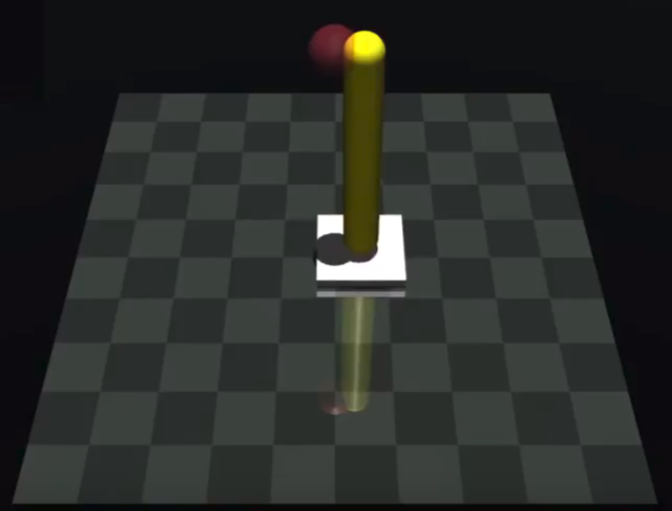
\includegraphics[width=\linewidth]{./Figures/pole_30_2.png}
    \caption{pole length:30cm, radius:2cm, mass:400g}
  \end{subfigure}
  \caption{Simulation setup in MuJoCo simulation}
  \label{fig:pole}
\end{figure}

In order to transfer the simulation to a physical system, a 3DOF robotic arm with a force sensor are implemented. Also, the simulation model parameters are set as close as possible to the physical system. For example, the standard deviation of the force sensor in the simulation is set as 0.03N because the actual sensor in the physical system is 0.06N. Furthermore, the initial angle of the pole is uniformly distributed in a range of -10deg to 10deg as it is impossible for human to put the pole in a exact right angle.  

\begin{figure}[h!]
  \centering
  \begin{subfigure}[b]{0.5\linewidth}
    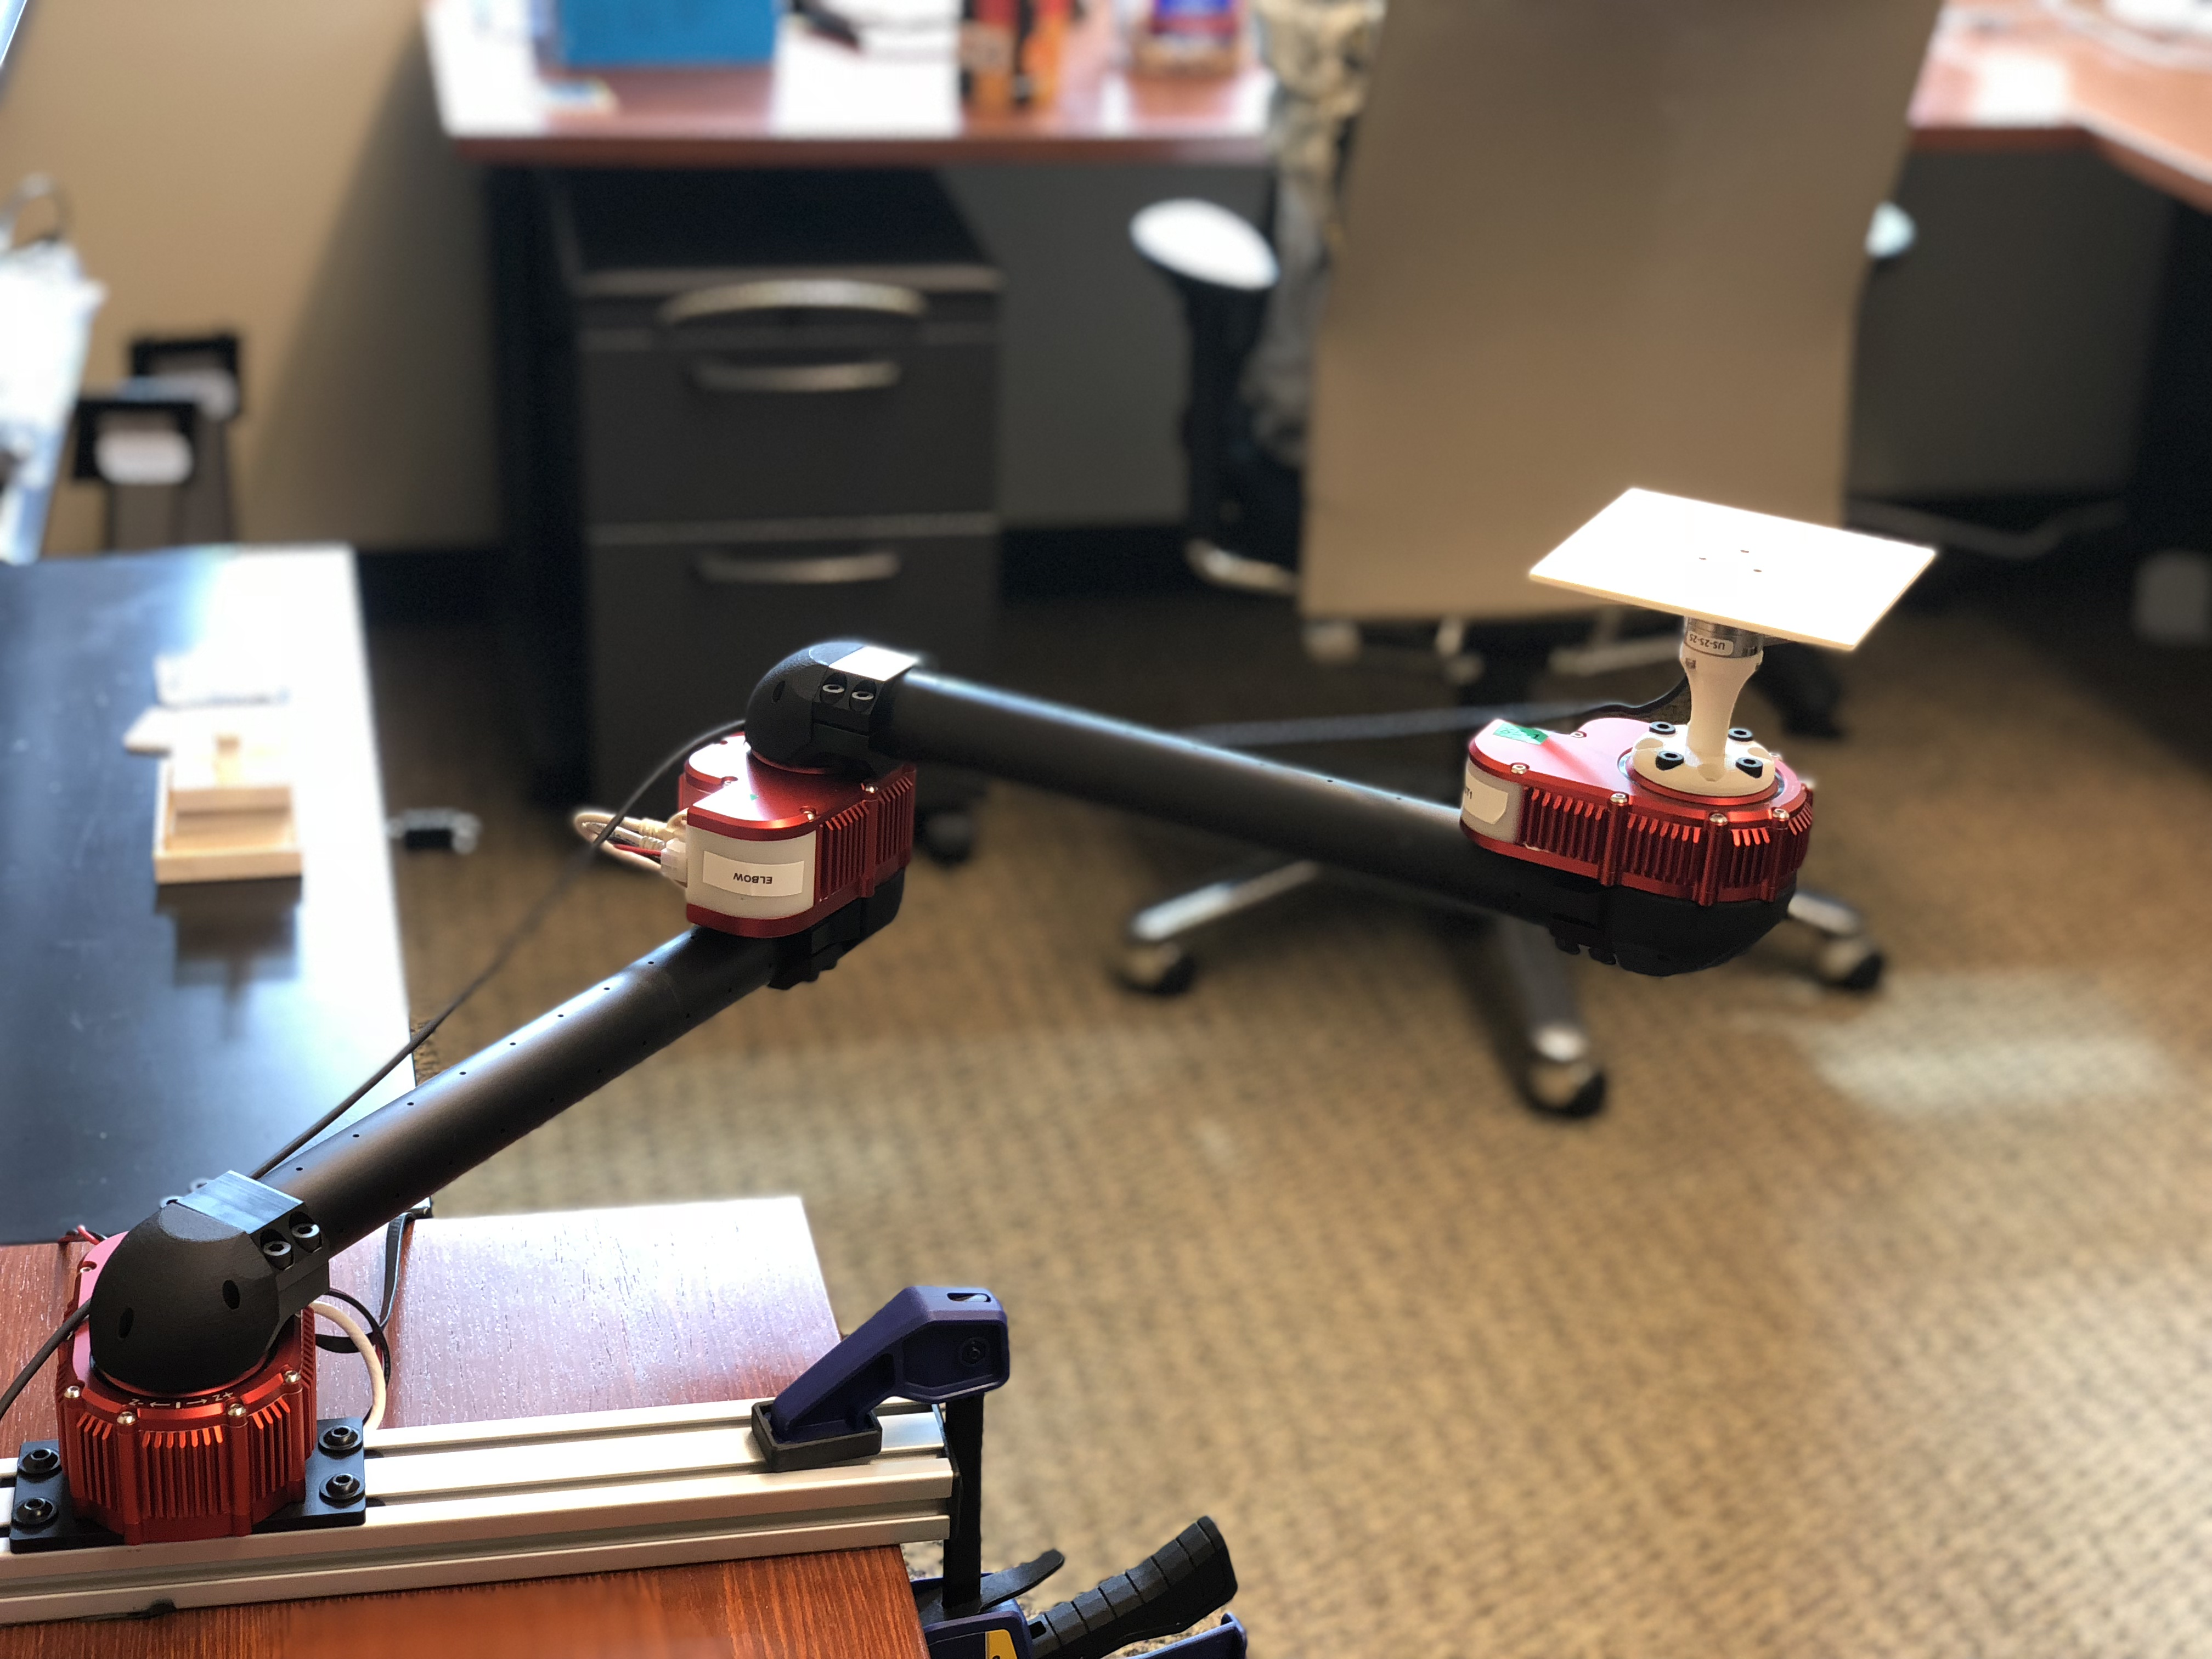
\includegraphics[width=\linewidth]{./Figures/balancer_arm.jpg}
    \caption{3DOF arm for the actuation of the balancer}
  \end{subfigure}
  \begin{subfigure}[b]{0.4\linewidth}
    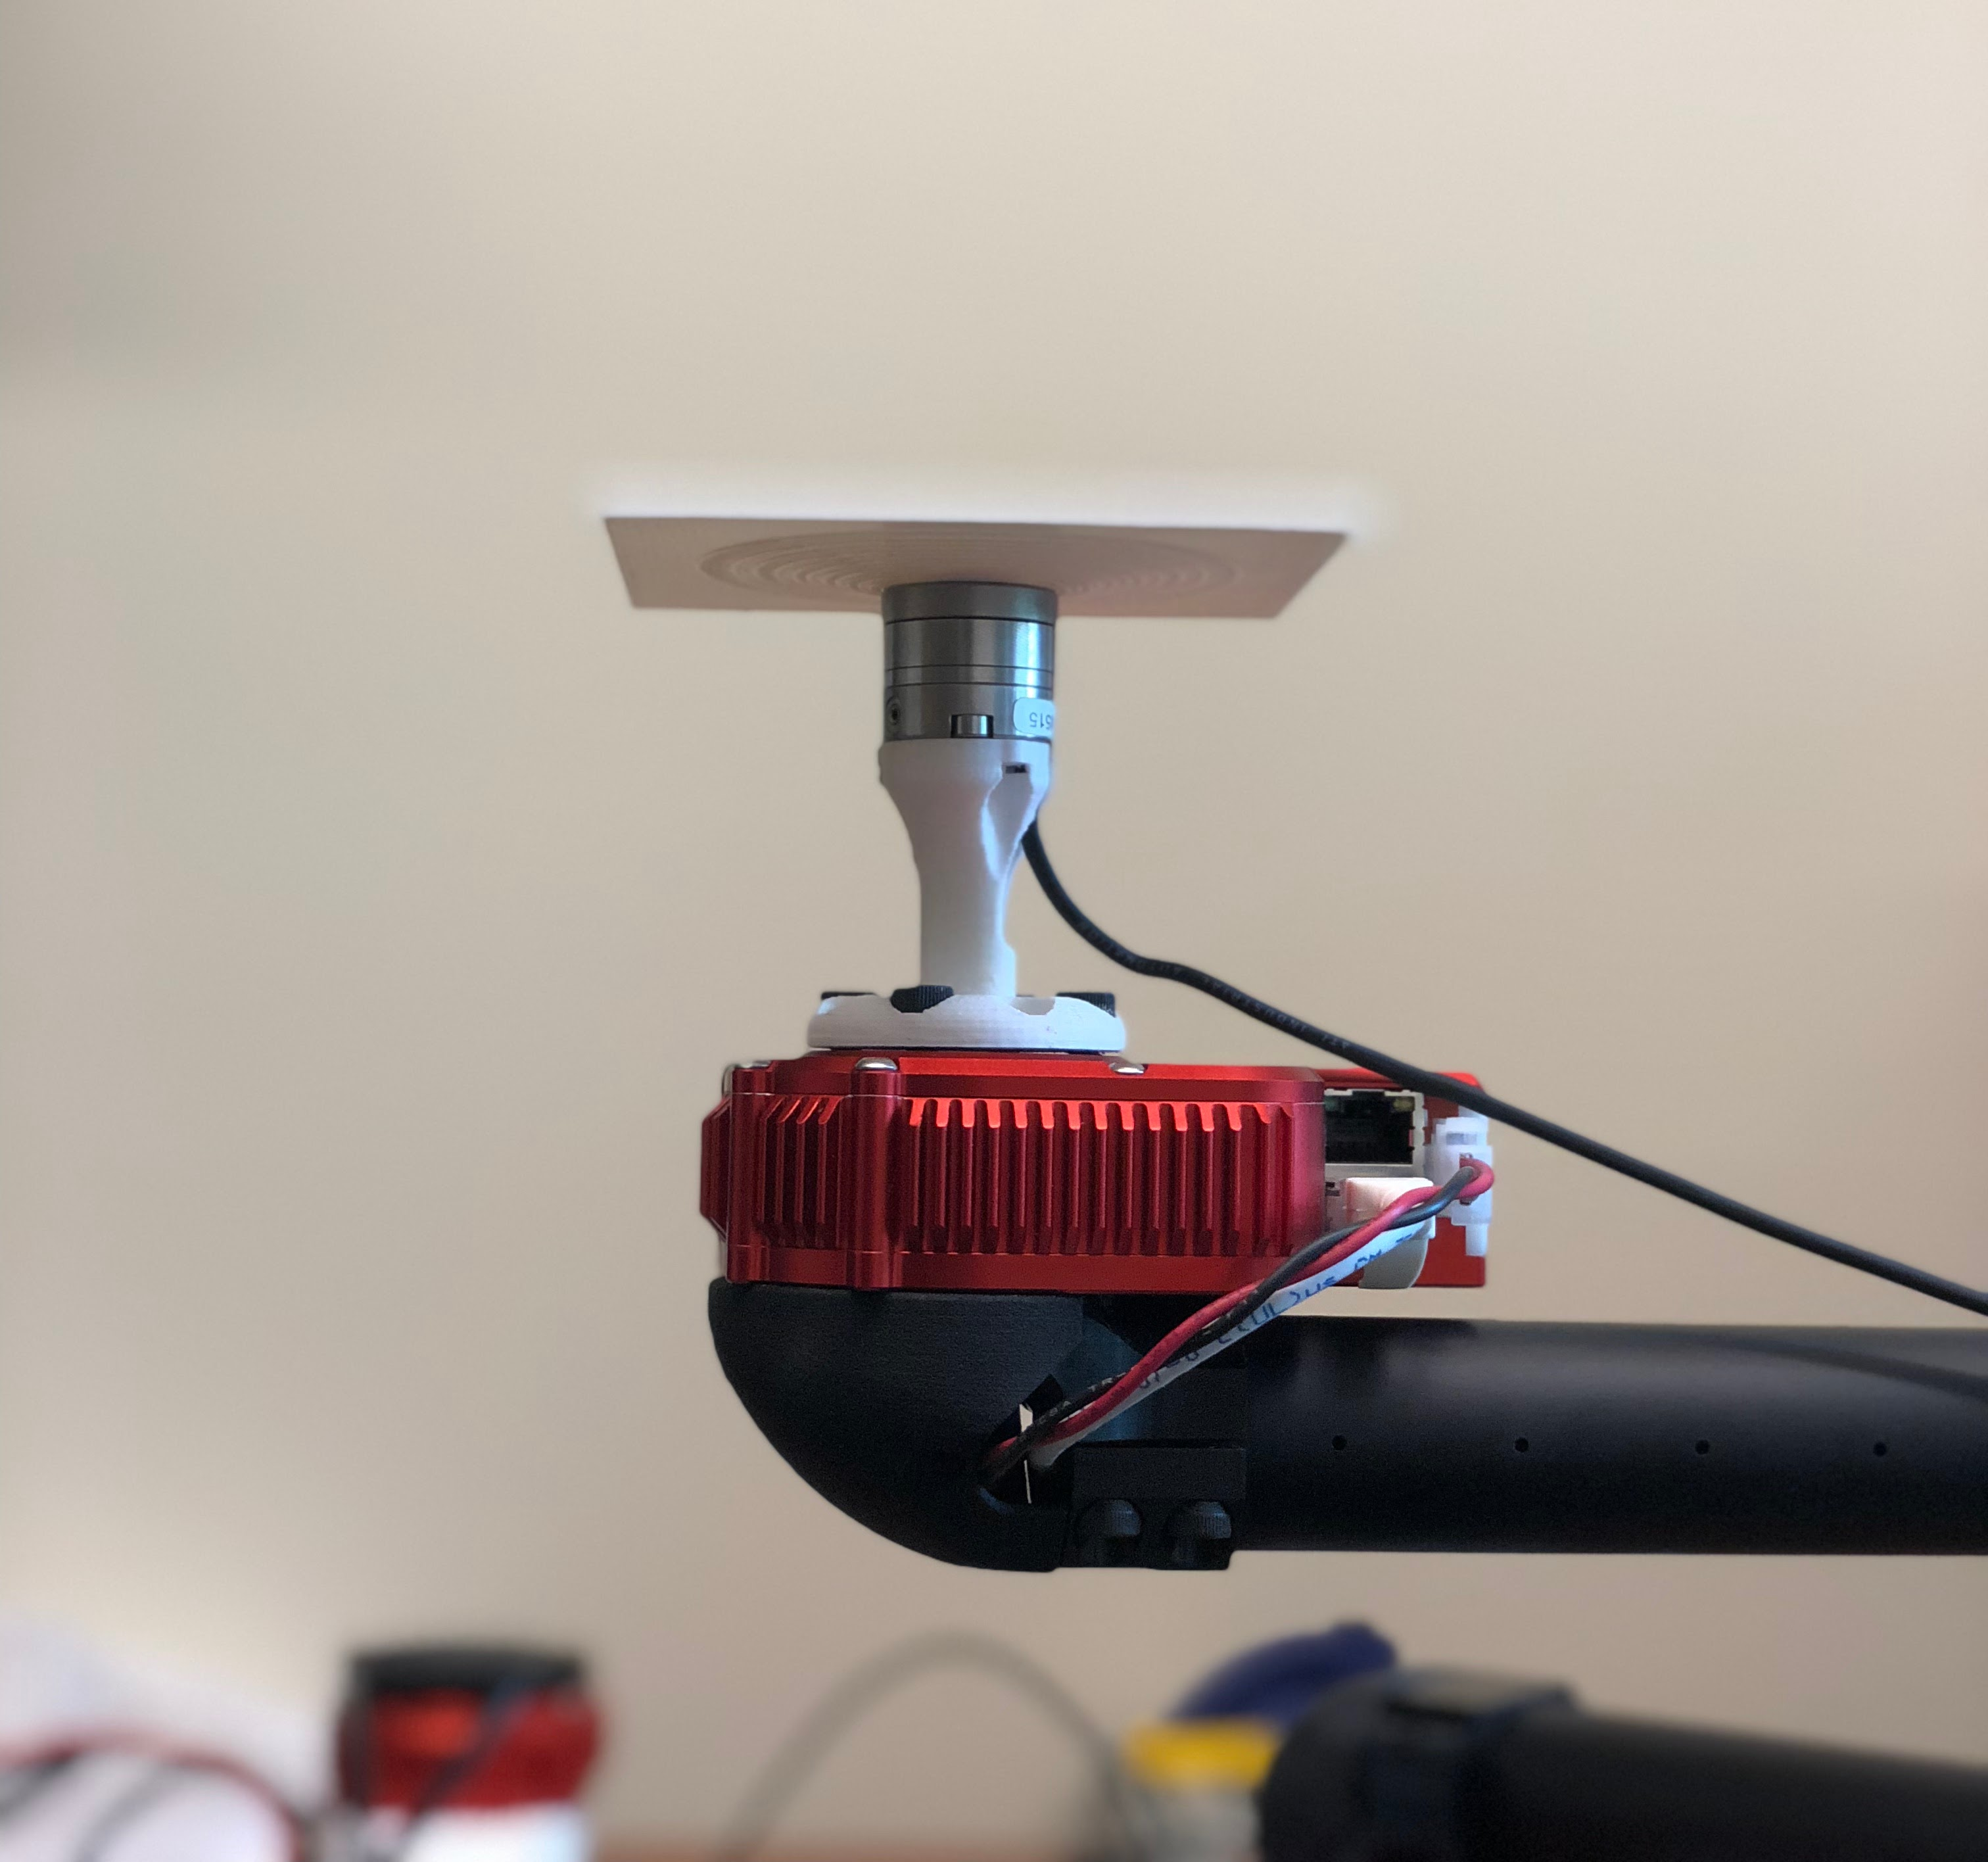
\includegraphics[width=\linewidth]{./Figures/balancer_sensor.jpg}
    \caption{Installation of the force sensor}
  \end{subfigure}
  \caption{Physical system implementation}
  \label{fig:pole}
\end{figure}

%\subsection{Physical System}

\section{Result}

Learning parameters, such as the number of iterations, trajectories, and episodes are adjusted depending on the physical parameters of the pole and the balancer to make the learning converging. For the pole with 30cm length, 1,2cm radius, and 400g, the number of iterations is 600, the number of trajectories is 250, and the maximum episode steps are 800. The gear of the motor and the time step are adjusted as well. Simulation parameters are shown in the below table.

\begin{table}[h!]
\centering
  \begin{center}
  \begin{tabular}{ |p{4cm}||p{2cm}|  }
  \hline
  \multicolumn{2}{|c|}{Simulation parameters} \\[0.5ex]
  \hline
  Number of iterations & 600\\
  Number of trajectories & 250\\
  Maximum episode steps & 800\\
  Timestep & 0.01\\
  Skip & 1\\
  \hline
  \end{tabular}
  \end{center}
  \caption{Simulation parameters}
  \label{table:1}
\end{table}

Rewards also have coefficients to give different weights. For example, the pole with 1cm radius has 20 for the angle rewards, 3 for the distance rewards and 3e-1 for the control cost penalty. Those coefficients are found manually.

Even though there are some steady state error in the position, the balancer was able to balance the pole.


\section{Discussion}

There are several aspects to improve such as the way to find the optimal values of learning parameters and rewards coefficients. In this paper, those numbers are found manually and takes long time. 

The physical system test is not performed in this paper due to the lack of time, this can be done in the near future. During the transfer from the simulation to the physical system, the latency of the system can be also an important factor to consider.  
%\subsection{Environment}

%\section{Conclusion}
%
%
%\section{References}

\end{document}